\documentclass[10pt]{beamer}

% Packages
\usepackage[utf8]{inputenc}
\usepackage[T1]{fontenc}
\usepackage{amsmath, amssymb, amsthm}
\usepackage{graphicx}
\usepackage{booktabs}
\usepackage{hyperref}
\usepackage{tikz}
\usetikzlibrary{trees, positioning, shapes, arrows.meta, patterns, decorations.pathreplacing}

\usepackage{algorithm}
\usepackage{algpseudocode}

% Theme settings
\usetheme{default}
\usecolortheme{default}
\usefonttheme{professionalfonts}

% Color definitions (minimalist academic palette)
\definecolor{ThemeBlue}{RGB}{0, 62, 116}
\definecolor{DarkGray}{RGB}{51, 51, 51}
\definecolor{LightGray}{RGB}{245, 245, 245}
\definecolor{AccentOrange}{RGB}{214, 96, 77}
\definecolor{AccentGreen}{RGB}{0, 128, 0}
\definecolor{LightBlue}{RGB}{200, 220, 240}
\definecolor{LightOrange}{RGB}{255, 220, 200}
\definecolor{LightGreen}{RGB}{200, 240, 200}

% Apply colors
\setbeamercolor{frametitle}{fg=ThemeBlue, bg=white}
\setbeamercolor{title}{fg=ThemeBlue}
\setbeamercolor{structure}{fg=ThemeBlue}
\setbeamercolor{normal text}{fg=DarkGray}
\setbeamercolor{block title}{fg=white, bg=ThemeBlue}
\setbeamercolor{block body}{fg=DarkGray, bg=LightGray}
\setbeamercolor{itemize item}{fg=ThemeBlue}
\setbeamercolor{enumerate item}{fg=ThemeBlue}

% Remove navigation symbols
\setbeamertemplate{navigation symbols}{}

% Customize frame title
\setbeamertemplate{frametitle}{
  \vspace{0.5em}
  \insertframetitle
  \vspace{0.3em}
}

% Customize itemize
\setbeamertemplate{itemize items}[circle]
\setlength{\leftmargini}{1.5em}

% Footer
\setbeamertemplate{footline}{
  \leavevmode%
  \hbox{%
  \begin{beamercolorbox}[wd=.333333\paperwidth,ht=2.25ex,dp=1ex,left]{author in head/foot}%
    \hspace{1em}\usebeamerfont{author in head/foot}\insertshortauthor
  \end{beamercolorbox}%
  \begin{beamercolorbox}[wd=.333333\paperwidth,ht=2.25ex,dp=1ex,center]{title in head/foot}%
    \usebeamerfont{title in head/foot}\insertshorttitle
  \end{beamercolorbox}%
  \begin{beamercolorbox}[wd=.333333\paperwidth,ht=2.25ex,dp=1ex,right]{date in head/foot}%
    \usebeamerfont{date in head/foot}\insertshortdate{}\hspace*{2em}
    \insertframenumber{} / \inserttotalframenumber\hspace*{2ex}
  \end{beamercolorbox}}%
  \vskip0pt%
}

% Title page customization
\setbeamertemplate{title page}{
  \vbox{}
  \vfill
  \begingroup
    \centering
    {\usebeamercolor[fg]{title}\usebeamerfont{title}\inserttitle\par}
    \vskip0.5em
    {\usebeamercolor[fg]{subtitle}\usebeamerfont{subtitle}\insertsubtitle\par}
    \vskip2em
    {\usebeamercolor[fg]{author}\usebeamerfont{author}\insertauthor\par}
    \vskip0.5em
    {\usebeamercolor[fg]{institute}\usebeamerfont{institute}\insertinstitute\par}
    \vskip1em
    {\usebeamercolor[fg]{date}\usebeamerfont{date}\insertdate\par}
  \endgroup
  \vfill
}

% Commands for highlighting
\newcommand{\highlight}[1]{\textcolor{AccentOrange}{\textbf{#1}}}
\newcommand{\emphbox}[1]{\colorbox{LightGray}{\textcolor{DarkGray}{#1}}}

% Mathematical operators
\DeclareMathOperator*{\argmin}{arg\,min}
\DeclareMathOperator*{\argmax}{arg\,max}
\DeclareMathOperator{\E}{\mathbb{E}}
\DeclareMathOperator{\Var}{Var}
\DeclareMathOperator{\Cov}{Cov}
\DeclareMathOperator{\Corr}{Corr}
\DeclareMathOperator{\tr}{tr}

%----------------------------------------------------------------------------------------
% TITLE PAGE
%----------------------------------------------------------------------------------------

\title{Big Data in Finance}
\subtitle{Week 5: Unsupervised Learning}
\author{Dr Daniele Bianchi}
\date{Spring 2026}

%----------------------------------------------------------------------------------------
% DOCUMENT
%----------------------------------------------------------------------------------------

\begin{document}

\AtBeginSection[]{
  \begin{frame}[plain]
    \vfill
    \begin{center}
      {\Large\color{ThemeBlue}\insertsection}
    \end{center}
    \vfill
  \end{frame}
}


% Title slide
\begin{frame}[plain]
  \titlepage
\end{frame}

% Outline slide
\begin{frame}{Today's Agenda}
  \tableofcontents
\end{frame}

%----------------------------------------------------------------------------------------
\section{From Supervised to Unsupervised Learning}
%----------------------------------------------------------------------------------------

\begin{frame}{Recap: What We've Learned So Far}

  \textbf{Supervised learning:} We had a target variable $Y$ to predict

  \vspace{1em}
  \begin{itemize}
    \item \textbf{Regression} (Weeks 2--3): Predict returns, continuous $Y$
    \begin{itemize}
      \item Ridge, Lasso, Random Forest, Boosting
    \end{itemize}

    \vspace{0.5em}
    \item \textbf{Classification} (Week 4): Predict default, binary $Y$
    \begin{itemize}
      \item Logistic regression, classification trees, ensembles
    \end{itemize}
  \end{itemize}

  \vspace{1em}
  \begin{block}{Common Structure}
    Given $(X_i, Y_i)$ pairs, learn $\widehat{f}$ such that $\widehat{Y} = \widehat{f}(X)$ predicts $Y$ well.
  \end{block}
\end{frame}

%----------------------------------------------------------------------------------------

\begin{frame}{What Is Unsupervised Learning?}

  \textbf{Key difference:} There is \highlight{no target variable} $Y$

  \vspace{1em}
  We only observe features $X_1, X_2, \ldots, X_p$ for each observation. The goal is to discover \highlight{structure} in the data.

  \vspace{1em}
  \textbf{Two main tasks:}
  \begin{enumerate}
    \item \textbf{Dimensionality reduction:} Find a smaller set of variables that captures most of the information
    \begin{itemize}
      \item Principal Component Analysis (PCA)
    \end{itemize}

    \vspace{0.5em}
    \item \textbf{Clustering:} Group similar observations together
    \begin{itemize}
      \item K-means, hierarchical clustering
    \end{itemize}
  \end{enumerate}

  \vspace{1em}
  \begin{block}{Today's Focus}
    PCA for dimensionality reduction; clustering for segmentation
  \end{block}
\end{frame}

%----------------------------------------------------------------------------------------

\begin{frame}{Why Does This Matter in Finance?}

  \textbf{Dimensionality reduction (PCA):}
  \begin{itemize}
    \item \textit{Factor models:} Extract common factors from many asset returns
    \item \textit{Feature reduction:} 100+ characteristics $\to$ few principal components
    \item \textit{Noise reduction:} Remove idiosyncratic variation
    \item \textit{Multicollinearity:} Predictors often highly correlated
  \end{itemize}

  \vspace{1em}
  \textbf{Clustering:}
  \begin{itemize}
    \item \textit{Portfolio construction:} Group similar stocks
    \item \textit{Regime detection:} Identify market states (bull/bear/crisis)
    \item \textit{Client segmentation:} Risk profiles, investment preferences
    \item \textit{Peer analysis:} Find comparable firms
  \end{itemize}

  \vspace{0.5em}
  \begin{block}{Key Insight}
    Unsupervised methods help us understand \highlight{structure} before (or instead of) prediction
  \end{block}
\end{frame}

%----------------------------------------------------------------------------------------

\begin{frame}{A Motivating Example: Stock Returns}

  \textbf{Setting:} We observe monthly returns for 500 stocks over 10 years

  \vspace{0.5em}
  \begin{itemize}
    \item Data matrix: $500 \times 120$ (stocks $\times$ months)
    \item Each row is a stock's return time series
  \end{itemize}

  \vspace{1em}
  \textbf{Observation:} Stock returns are highly correlated!
  \begin{itemize}
    \item When the market goes up, most stocks go up
    \item Tech stocks move together, banks move together, etc.
  \end{itemize}

  \vspace{1em}
  \textbf{Questions we can ask:}
  \begin{enumerate}
    \item What are the common factors? (PCA)
    \item Can we group stocks into similar ``clusters''? (Clustering)
  \end{enumerate}
\end{frame}

%----------------------------------------------------------------------------------------
\section{Principal Component Analysis (PCA)}
%----------------------------------------------------------------------------------------

\begin{frame}{The Core Idea of PCA}

  \textbf{Goal:} Find new variables (``principal components'') that:
  \begin{enumerate}
    \item Are \highlight{linear combinations} of the original variables
    \item Capture as much \highlight{variance} as possible
    \item Are \highlight{uncorrelated} with each other
  \end{enumerate}

  \vspace{1em}
  \textbf{Why variance?}
  \begin{itemize}
    \item Variance $=$ information (variables that don't vary carry no information)
    \item PCA finds directions of maximum spread in the data
  \end{itemize}

  \vspace{1em}
  \textbf{Intuition:} If we can only keep $k < p$ dimensions, which ones preserve the most information about the original data?

  \vspace{0.5em}
  \begin{block}{Key Result}
    PCA gives us the \emph{optimal} linear dimensionality reduction in terms of preserved variance
  \end{block}
\end{frame}

%----------------------------------------------------------------------------------------

\begin{frame}{Geometric Intuition: 2D Example}

  \textbf{Imagine data in 2D:} Points scattered in an ellipse

  \vspace{0.5em}
  \begin{center}
  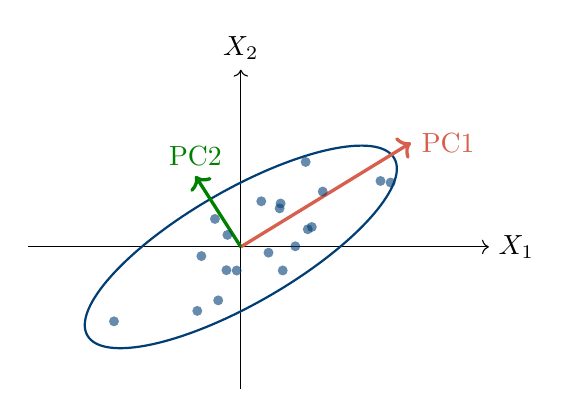
\begin{tikzpicture}[scale=0.9]
    % Axes
    \draw[->] (-3,0) -- (3.5,0) node[right] {$X_1$};
    \draw[->] (0,-2) -- (0,2.5) node[above] {$X_2$};

    % Draw ellipse of data points
    \draw[ThemeBlue, thick, rotate=30] (0,0) ellipse (2.5cm and 0.8cm);

    % First PC (major axis)
    \draw[->, AccentOrange, very thick] (0,0) -- (2.4,1.47) node[right] {PC1};

    % Second PC (minor axis)
    \draw[->, AccentGreen, very thick] (0,0) -- (-0.64,1) node[above] {PC2};

    % Scatter some points
    \foreach \i in {1,...,20} {
      \pgfmathsetmacro{\a}{rand*2.3}
      \pgfmathsetmacro{\b}{rand*0.6}
      \pgfmathsetmacro{\x}{\a*cos(30) - \b*sin(30)}
      \pgfmathsetmacro{\y}{\a*sin(30) + \b*cos(30)}
      \fill[ThemeBlue, opacity=0.6] (\x,\y) circle (2pt);
    }
  \end{tikzpicture}
  \end{center}

  \vspace{0.3em}
  \begin{itemize}
    \item \textcolor{AccentOrange}{\textbf{PC1:}} Direction of maximum variance (major axis)
    \item \textcolor{AccentGreen}{\textbf{PC2:}} Orthogonal direction, captures remaining variance
    \item If we project onto PC1 only, we lose the least information
  \end{itemize}
\end{frame}

%----------------------------------------------------------------------------------------

\begin{frame}{The Mathematics of PCA}

  \textbf{Setup:} Data matrix $\mathbf{X}$ is $n \times p$ (observations $\times$ variables)

  \vspace{0.5em}
  Assume variables are \highlight{centered} (mean zero).

  \vspace{1em}
  \textbf{First principal component:}
  \begin{itemize}
    \item Find loadings $\mathbf{w}_1 = (w_{11}, w_{12}, \ldots, w_{1p})^\top$ with $\|\mathbf{w}_1\| = 1$
    \item Such that the new variable $Z_1 = \mathbf{X}\mathbf{w}_1$ has \highlight{maximum variance}
  \end{itemize}

  \[
  \mathbf{w}_1 = \argmax_{\|\mathbf{w}\|=1} \Var(Z_1) = \argmax_{\|\mathbf{w}\|=1} \mathbf{w}^\top \mathbf{S} \mathbf{w}
  \]

  where $\mathbf{S} = \frac{1}{n-1}\mathbf{X}^\top\mathbf{X}$ is the sample covariance matrix.

  \vspace{1em}
  \textbf{Second principal component:} Same, but require $Z_2 \perp Z_1$ (uncorrelated with first)

  \vspace{0.5em}
  And so on for PC3, PC4, $\ldots$
\end{frame}

%----------------------------------------------------------------------------------------

\begin{frame}{How Does PCA Find the Components?}

\textbf{The algorithm:} PCA analyzes the covariance matrix of your data

\vspace{1em}
\textbf{What you need to know:}
\begin{enumerate}
   \item PCA finds the \highlight{directions} (principal components) where data varies most
    \item Each direction comes with a \highlight{number} (eigenvalue) measuring its importance
   \item Directions are ranked: PC1 captures most variance, PC2 second-most, etc.
    \item Directions are \highlight{perpendicular} to each other (uncorrelated)
  \end{enumerate}

  \vspace{1em}
  \textbf{The outputs:}
  \begin{itemize}
    \item \textbf{Loadings:} How much each original variable contributes to each PC
    \item \textbf{Eigenvalues:} How much variance each PC captures
    \item \textbf{Scores:} The new transformed data points
  \end{itemize}

  \vspace{0.5em}
  \begin{block}{Good News}
    Python handles all the math --- you just need to interpret the results!
  \end{block}
\end{frame}

\begin{frame}{How Much Information Do We Keep?}

  \textbf{Question:} If we reduce from $p$ variables to $k$ PCs, how much do we lose?

  \vspace{1em}
  \textbf{Think of it this way:}
  \begin{itemize}
    \item Total variance $=$ total ``information'' in your data
    \item Each PC captures some fraction of this information
    \item PC1 captures the most, PC2 second-most, and so on
  \end{itemize}

  \vspace{1em}
  \textbf{Example:} 10 stock returns, applying PCA

 \vspace{0.3em}
  \begin{center}
  \begin{tabular}{lcc}
    \toprule
    & \textbf{Variance Explained} & \textbf{Cumulative} \\
    \midrule
    PC1 & 45\% & 45\% \\
    PC2 & 20\% & 65\% \\
    PC3 & 10\% & 75\% \\
    PCs 4--10 & 25\% & 100\% \\
    \bottomrule
  \end{tabular}
  \end{center}

  \vspace{0.5em}
 \textbf{Interpretation:} Using just 3 PCs instead of 10 variables, we retain 75\% of the information. The last 7 PCs add little --- mostly noise.
\end{frame}

%----------------------------------------------------------------------------------------

\begin{frame}{The Scree Plot: Choosing Number of Components}

  \highlight{How many PCs should we keep?}

  \vspace{0.5em}
  \begin{center}
  \begin{tikzpicture}[scale=0.8]
    % Axes
    \draw[->] (0,0) -- (8,0) node[right] {Component};
    \draw[->] (0,0) -- (0,5) node[above] {Eigenvalue};

    % Eigenvalues (declining)
    \draw[thick, ThemeBlue, mark=*] plot coordinates {(1,4.2) (2,1.8) (3,0.7) (4,0.45) (5,0.3) (6,0.2) (7,0.15)};

    % Points
    \foreach \x/\y in {1/4.2, 2/1.8, 3/0.7, 4/0.45, 5/0.3, 6/0.2, 7/0.15} {
      \fill[ThemeBlue] (\x,\y) circle (3pt);
    }

    % Elbow annotation
    \draw[dashed, AccentOrange] (3,0) -- (3,2.5);
    \node[AccentOrange, below] at (3,0) {\small ``Elbow''};

    % Labels
    \node[below] at (1,0) {1};
    \node[below] at (4,0) {4};
    \node[below] at (7,0) {7};
  \end{tikzpicture}
  \end{center}

  \vspace{0.3em}
  \textbf{Common approaches:}
  \begin{enumerate}
    \item \textit{Elbow method:} Look for ``elbow'' where curve flattens
    \item \textit{Cumulative variance:} Keep enough for 80--90\% CPVE
    \item \textit{Cross-validation:} If using PCs for prediction, tune $k$ via CV
  \end{enumerate}
\end{frame}

%----------------------------------------------------------------------------------------

\begin{frame}{Standardization: An Important Choice}

  \textbf{Question:} Should we standardize variables before PCA?

  \vspace{1em}
  \textbf{Without standardization:}
  \begin{itemize}
    \item Use covariance matrix $\mathbf{S}$
    \item Variables with larger variance dominate
    \item Appropriate when scale is homogeneous (e.g., all returns in \%)
  \end{itemize}

  \vspace{0.5em}
  \textbf{With standardization:}
  \begin{itemize}
    \item Use correlation matrix $\mathbf{R}$ (standardize each variable to variance 1)
    \item All variables treated equally regardless of scale
    \item Appropriate when scales differ (e.g., mixed financial ratios)
  \end{itemize}

  \vspace{1em}
  \begin{block}{Rule of Thumb}
    If variables are in different units or have very different variances, \highlight{standardize first}. If all variables are comparable (e.g., stock returns), covariance may be preferred.
  \end{block}
\end{frame}

%----------------------------------------------------------------------------------------

\begin{frame}{Interpreting Principal Components}

  \textbf{The loadings} (eigenvector entries) tell us what each PC represents

  \vspace{1em}
  \textbf{Example:} PCA on stock returns

  \vspace{0.5em}
  \begin{center}
  \begin{tabular}{lccc}
    \toprule
    \textbf{Stock} & \textbf{PC1 Loading} & \textbf{PC2 Loading} & \textbf{PC3 Loading} \\
    \midrule
    Apple & 0.15 & 0.35 & $-0.10$ \\
    Microsoft & 0.14 & 0.32 & $-0.12$ \\
    JPMorgan & 0.12 & $-0.25$ & 0.40 \\
    Goldman Sachs & 0.11 & $-0.28$ & 0.38 \\
    ExxonMobil & 0.10 & $-0.05$ & $-0.30$ \\
    $\vdots$ & $\vdots$ & $\vdots$ & $\vdots$ \\
    \bottomrule
  \end{tabular}
  \end{center}

  \vspace{0.5em}
  \textbf{Interpretation:}
  \begin{itemize}
    \item \textbf{PC1:} All positive loadings $\approx$ ``market factor''
    \item \textbf{PC2:} Tech positive, banks negative $\approx$ ``growth vs.\ value''
    \item \textbf{PC3:} Banks positive, energy negative $\approx$ ``sector rotation''
  \end{itemize}
\end{frame}

%----------------------------------------------------------------------------------------

\begin{frame}{PCA as a Factor Model}

  \textbf{Connection to finance:} PCA extracts \highlight{statistical factors}

  \vspace{1em}
  \textbf{Factor model representation:}
  \[
  R_{it} = \alpha_i + \beta_{i1} F_{1t} + \beta_{i2} F_{2t} + \cdots + \beta_{ik} F_{kt} + \varepsilon_{it}
  \]

  where:
  \begin{itemize}
    \item $F_{jt}$: Factor $j$ at time $t$ (the principal component scores)
    \item $\beta_{ij}$: Loading of asset $i$ on Factor $j$
    \item $\varepsilon_{it}$: Idiosyncratic return
  \end{itemize}

  \vspace{1em}
  \textbf{Key insight:} PCA on \emph{returns} gives us the factors that best explain return \emph{covariances}

  \vspace{0.5em}
  \begin{block}{Statistical vs.\ Economic Factors}
    PCA factors are \highlight{statistical} (maximize variance explained), not necessarily \highlight{economic} (like Fama-French). We'll compare them in the next lecture.
  \end{block}
\end{frame}

%----------------------------------------------------------------------------------------

\begin{frame}{Limitations of PCA}

  \highlight{PCA is powerful, but has limitations:}

  \vspace{1em}
  \begin{enumerate}
    \item \textbf{Linearity:} Only finds linear combinations
    \begin{itemize}
      \item Kernel PCA can capture non-linear structure
    \end{itemize}

    \vspace{0.5em}
    \item \textbf{Orthogonality:} Components must be uncorrelated
    \begin{itemize}
      \item Real factors may be correlated (e.g., value and momentum)
    \end{itemize}

    \vspace{0.5em}
    \item \textbf{Interpretability:} PCs are linear combinations of \emph{all} variables
    \begin{itemize}
      \item Sparse PCA forces some loadings to zero
    \end{itemize}

    \vspace{0.5em}
    \item \textbf{Sample dependence:} Factors are estimated from data
    \begin{itemize}
      \item Can be unstable with small samples or noisy data
    \end{itemize}
  \end{enumerate}
\end{frame}

%----------------------------------------------------------------------------------------
\section{Clustering Methods}
%----------------------------------------------------------------------------------------

\begin{frame}{From Dimensionality Reduction to Clustering}

  \textbf{PCA:} Reduce the number of \emph{variables}

  \vspace{0.5em}
  \textbf{Clustering:} Group \emph{observations} into similar clusters

  \vspace{1em}
  \begin{center}
  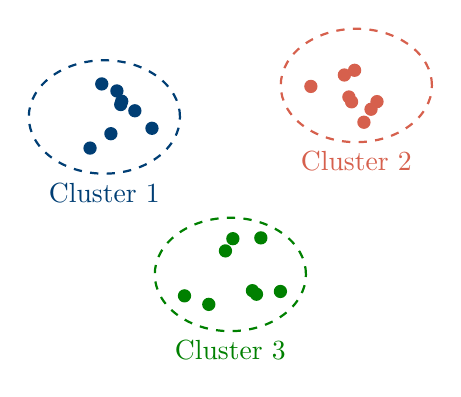
\begin{tikzpicture}[scale=0.8]
    % Cluster 1
    \foreach \i in {1,...,8} {
      \pgfmathsetmacro{\x}{-2 + rand*0.8}
      \pgfmathsetmacro{\y}{1.5 + rand*0.6}
      \fill[ThemeBlue] (\x,\y) circle (3pt);
    }
    \draw[ThemeBlue, dashed, thick] (-2,1.5) ellipse (1.2cm and 0.9cm);
    \node[ThemeBlue] at (-2,0.3) {Cluster 1};

    % Cluster 2
    \foreach \i in {1,...,8} {
      \pgfmathsetmacro{\x}{2 + rand*0.8}
      \pgfmathsetmacro{\y}{2 + rand*0.6}
      \fill[AccentOrange] (\x,\y) circle (3pt);
    }
    \draw[AccentOrange, dashed, thick] (2,2) ellipse (1.2cm and 0.9cm);
    \node[AccentOrange] at (2,0.8) {Cluster 2};

    % Cluster 3
    \foreach \i in {1,...,8} {
      \pgfmathsetmacro{\x}{0 + rand*0.8}
      \pgfmathsetmacro{\y}{-1 + rand*0.6}
      \fill[AccentGreen] (\x,\y) circle (3pt);
    }
    \draw[AccentGreen, dashed, thick] (0,-1) ellipse (1.2cm and 0.9cm);
    \node[AccentGreen] at (0,-2.2) {Cluster 3};
  \end{tikzpicture}
  \end{center}

  \vspace{0.3em}
  \textbf{Goal:} Find groups where observations within a cluster are similar, and observations in different clusters are dissimilar.
\end{frame}

%----------------------------------------------------------------------------------------

\begin{frame}{Applications of Clustering in Finance}

  \textbf{1. Portfolio construction:}
  \begin{itemize}
    \item Group stocks by return behavior (not just sector labels)
    \item Diversify by picking from different clusters
  \end{itemize}

  \vspace{0.5em}
  \textbf{2. Regime detection:}
  \begin{itemize}
    \item Cluster time periods by market conditions
    \item Identify bull markets, bear markets, crisis periods
  \end{itemize}

  \vspace{0.5em}
  \textbf{3. Client segmentation:}
  \begin{itemize}
    \item Group investors by risk tolerance, behavior
    \item Tailor products and advice
  \end{itemize}

  \vspace{0.5em}
  \textbf{4. Peer group analysis:}
  \begin{itemize}
    \item Find comparable companies for valuation
    \item Data-driven alternative to SIC codes
  \end{itemize}
\end{frame}

%----------------------------------------------------------------------------------------

\begin{frame}{K-Means Clustering: The Idea}

  \textbf{Goal:} Partition $n$ observations into $K$ clusters

  \vspace{1em}
  \textbf{Objective:} Minimize within-cluster variation
  \[
  \min_{C_1, \ldots, C_K} \sum_{k=1}^{K} W(C_k)
  \]

  where $W(C_k) = \frac{1}{|C_k|} \sum_{i, j \in C_k} \|x_i - x_j\|^2$ is the within-cluster sum of squares.

  \vspace{1em}
  \textbf{Equivalently:}
  \[
  \min_{C_1, \ldots, C_K} \sum_{k=1}^{K} \sum_{i \in C_k} \|x_i - \mu_k\|^2
  \]

  where $\mu_k = \frac{1}{|C_k|} \sum_{i \in C_k} x_i$ is the centroid of cluster $k$.

  \vspace{0.5em}
  \begin{block}{Intuition}
    Find $K$ centroids and assign each point to nearest centroid
  \end{block}
\end{frame}

%----------------------------------------------------------------------------------------

\begin{frame}{K-Means Algorithm}

  \textbf{The algorithm:}

  \vspace{0.5em}
  \begin{enumerate}
    \item \textbf{Initialize:} Randomly assign each observation to one of $K$ clusters

    \vspace{0.3em}
    \item \textbf{Repeat until convergence:}
    \begin{enumerate}
      \item[(a)] \textbf{Update centroids:} Compute the mean of each cluster
      \[
      \mu_k = \frac{1}{|C_k|} \sum_{i \in C_k} x_i
      \]

      \item[(b)] \textbf{Reassign:} Assign each observation to the cluster with the closest centroid
      \[
      C(i) = \argmin_{k} \|x_i - \mu_k\|^2
      \]
    \end{enumerate}

    \vspace{0.3em}
    \item \textbf{Stop:} When assignments no longer change
  \end{enumerate}

  \vspace{1em}
  \textbf{Properties:}
  \begin{itemize}
    \item Guaranteed to decrease objective at each step
    \item Converges to a \highlight{local} minimum (not necessarily global)
    \item Run multiple times with different initializations
  \end{itemize}
\end{frame}

%----------------------------------------------------------------------------------------

\begin{frame}{K-Means: Visualization}

  \begin{center}
 \begin{figure}[p]
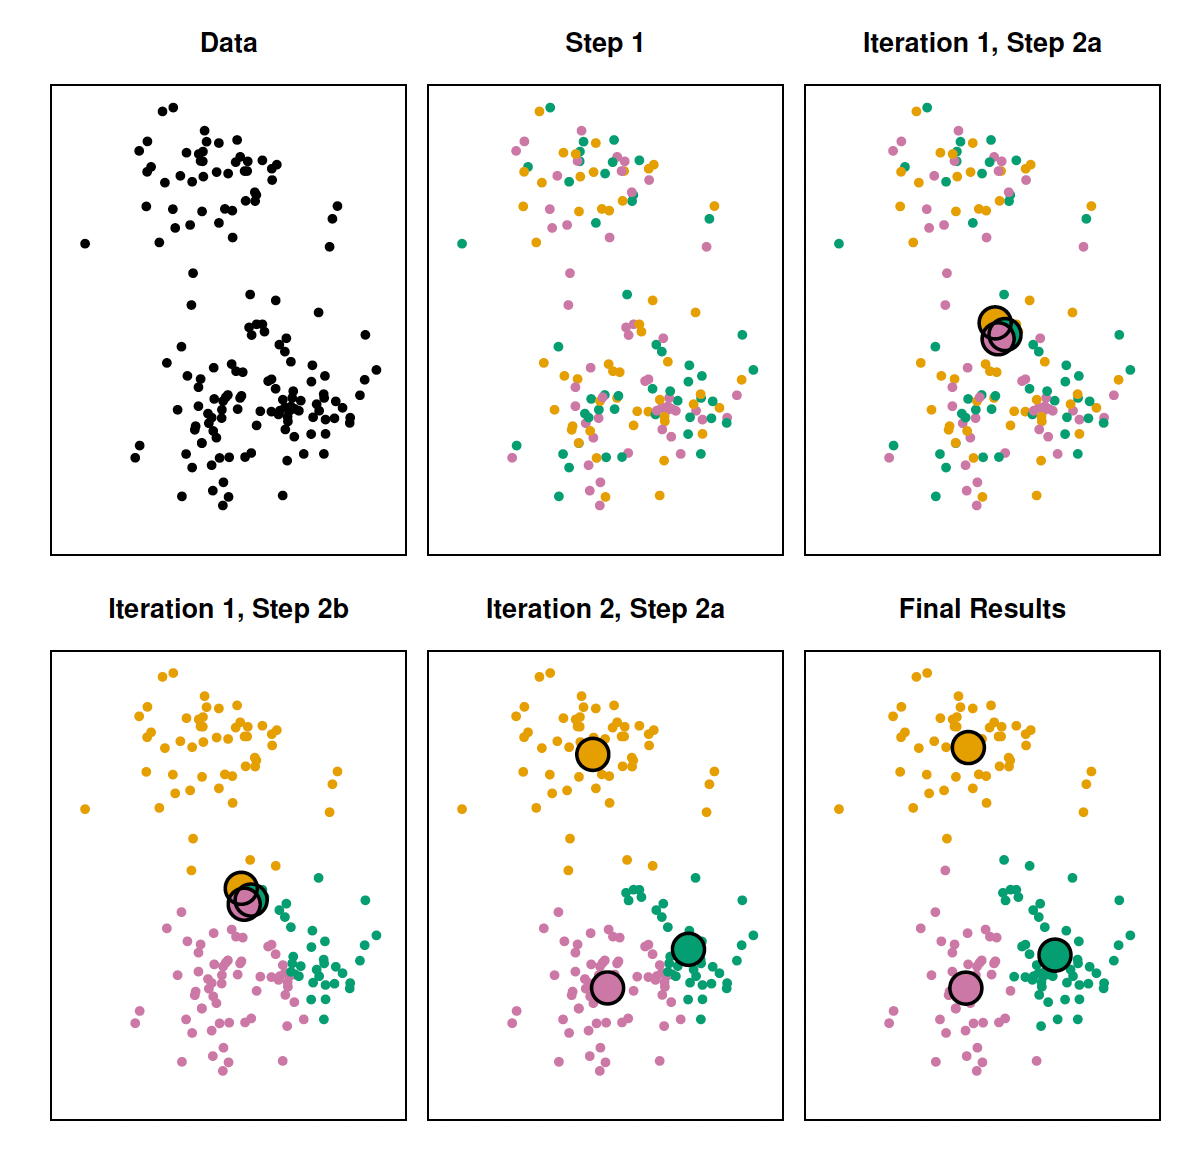
\includegraphics[width=.6\textwidth]{Figures/Fig022.png}
\end{figure}
  \end{center}

  \vspace{0.5em}
  The algorithm alternates between:
  \begin{itemize}
    \item Assigning points to the nearest centroid
    \item Recomputing centroids based on assignments
  \end{itemize}
\end{frame}

%----------------------------------------------------------------------------------------

\begin{frame}{Choosing the Number of Clusters $K$}

  \textbf{Problem:} K-means requires us to specify $K$ in advance

  \vspace{1em}
  \textbf{1. Elbow method:}
  \begin{itemize}
    \item Plot total within-cluster sum of squares vs.\ $K$
    \item Look for ``elbow'' where improvement slows
  \end{itemize}

  \vspace{0.5em}
  \begin{center}
  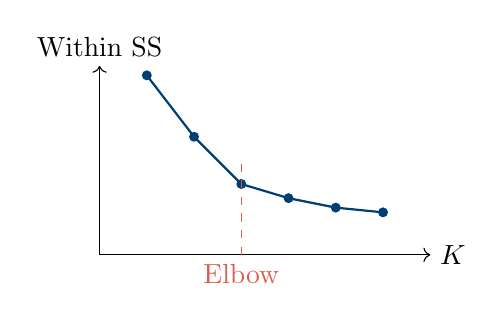
\begin{tikzpicture}[scale=0.6]
    \draw[->] (0,0) -- (7,0) node[right] {$K$};
    \draw[->] (0,0) -- (0,4) node[above] {Within SS};
    \draw[thick, ThemeBlue] plot coordinates {(1,3.8) (2,2.5) (3,1.5) (4,1.2) (5,1.0) (6,0.9)};
    \foreach \x/\y in {1/3.8, 2/2.5, 3/1.5, 4/1.2, 5/1.0, 6/0.9} {
      \fill[ThemeBlue] (\x,\y) circle (3pt);
    }
    \draw[dashed, AccentOrange] (3,0) -- (3,2);
    \node[below, AccentOrange] at (3,0) {Elbow};
  \end{tikzpicture}
  \end{center}

  \vspace{0.3em}
  \textbf{2. Domain knowledge:} In finance, often have natural groupings (sectors, regimes, anomalies)
\end{frame}

%----------------------------------------------------------------------------------------

\begin{frame}{Hierarchical Clustering}

  \textbf{Alternative approach:} Build a hierarchy of clusters

  \vspace{1em}
  \textbf{Agglomerative (bottom-up):}
  \begin{enumerate}
    \item Start: Each observation is its own cluster
    \item Merge: Combine the two closest clusters
    \item Repeat until all observations are in one cluster
  \end{enumerate}

  \vspace{1em}
  \textbf{Result:} A \highlight{dendrogram} showing the merging sequence

  \vspace{0.5em}
  \begin{center}
  \begin{tikzpicture}[scale=0.7]
    % Leaves
    \foreach \x/\n in {0/A, 1/B, 2/C, 3/D, 4/E} {
      \node at (\x,0) {\small \n};
      \draw (\x,0.3) -- (\x,0.5);
    }
    % First merge
    \draw (0,0.5) -- (0,1) -- (1,1) -- (1,0.5);
    \draw (0.5,1) -- (0.5,1.5);
    % Second merge
    \draw (2,0.5) -- (2,0.8) -- (3,0.8) -- (3,0.5);
    \draw (2.5,0.8) -- (2.5,2);
    % Third merge
    \draw (4,0.5) -- (4,2) -- (2.5,2);
    \draw (3.25,2) -- (3.25,2.5);
    % Final merge
    \draw (0.5,1.5) -- (0.5,3) -- (3.25,3) -- (3.25,2.5);

    % Height axis
    \draw[->] (-0.8,0) -- (-0.8,3.5) node[above] {\small Height};
  \end{tikzpicture}
  \end{center}

  \textbf{Advantage:} Don't need to pre-specify $K$; cut dendrogram at desired height
\end{frame}

%----------------------------------------------------------------------------------------

\begin{frame}{Linkage Methods}

  \highlight{How do we define ``distance'' between clusters?}

  \vspace{1em}
  \begin{center}
  \begin{tabular}{lp{7cm}}
    \toprule
    \textbf{Linkage} & \textbf{Definition} \\
    \midrule
    Single & Minimum distance between any two points \\
    \addlinespace
    Complete & Maximum distance between any two points \\
    \addlinespace
    Average & Average distance between all pairs \\
    \addlinespace
    Ward & Increase in within-cluster variance after merging \\
    \bottomrule
  \end{tabular}
  \end{center}

  \vspace{1em}
  \textbf{Recommendations:}
  \begin{itemize}
    \item \textbf{Ward:} Tends to produce compact, equal-sized clusters (often best)
    \item \textbf{Complete:} Produces compact clusters
    \item \textbf{Single:} Can create long ``chains'' (often problematic)
  \end{itemize}
\end{frame}

%----------------------------------------------------------------------------------------

\begin{frame}{K-Means vs.\ Hierarchical: Trade-offs}

  \begin{center}
  \begin{tabular}{lcc}
    \toprule
    & \textbf{K-Means} & \textbf{Hierarchical} \\
    \midrule
    Specify $K$? & Yes, in advance & No (cut dendrogram) \\
    \addlinespace
    Scalability & $O(nKt)$ --- fast & $O(n^2)$ or $O(n^3)$ --- slow \\
    \addlinespace
    Cluster shape & Spherical & Flexible \\
    \addlinespace
    Deterministic? & No (random init) & Yes \\
    \addlinespace
    Hierarchical structure? & No & Yes (dendrogram) \\
    \bottomrule
  \end{tabular}
  \end{center}

  \vspace{1em}
  \textbf{In practice:}
  \begin{itemize}
    \item K-means: Large datasets, when $K$ is known or tunable
    \item Hierarchical: Smaller datasets, want to explore structure, interpretability
    \item Often: Use hierarchical for exploration, K-means for final clustering
  \end{itemize}
\end{frame}

%----------------------------------------------------------------------------------------

\begin{frame}{Important Considerations for Clustering}

  \textbf{1. Feature scaling:}
  \begin{itemize}
    \item Clustering uses distances --- scale matters!
    \item Usually standardize features before clustering
  \end{itemize}

  \vspace{0.5em}
  \textbf{2. Dimensionality:}
  \begin{itemize}
    \item High dimensions $\Rightarrow$ distances become less meaningful
    \item Consider PCA before clustering (``spectral clustering'' approach)
  \end{itemize}

  \vspace{0.5em}
  \textbf{3. Outliers:}
  \begin{itemize}
    \item K-means sensitive to outliers (affects centroids)
    \item Consider robust alternatives or remove outliers first
  \end{itemize}

  \vspace{0.5em}
  \textbf{4. Validation:}
  \begin{itemize}
    \item No ``ground truth'' in unsupervised learning
    \item Use multiple methods, check stability, domain validation
  \end{itemize}
\end{frame}

%----------------------------------------------------------------------------------------
\section{Recap: PCA and Clustering}
%----------------------------------------------------------------------------------------

\begin{frame}{What We Learned in Part I}

  \textbf{Principal Component Analysis:}
  \begin{itemize}
    \item Find linear combinations that maximize variance
    \item Eigenvalue decomposition of covariance matrix
    \item First few PCs often capture most variation
    \item Standardization matters when scales differ
  \end{itemize}

  \vspace{1em}
  \textbf{Clustering:}
  \begin{itemize}
    \item K-means: Partition into $K$ groups, minimize within-cluster variance
    \item Hierarchical: Build dendrogram, cut at desired level
    \item Validation: Elbow method, silhouette score
  \end{itemize}

  \vspace{1em}
  \begin{block}{Today's Focus}
    How do we apply these methods to \highlight{real financial problems}?
  \end{block}
\end{frame}

%----------------------------------------------------------------------------------------
\section{PCA for Statistical Factor Models}
%----------------------------------------------------------------------------------------

\begin{frame}{The Factor Model Framework}

  \textbf{Classic asset pricing:} Returns are driven by common factors
  \[
  R_{it} - R_f = \alpha_i + \beta_{i1} F_{1t} + \beta_{i2} F_{2t} + \cdots + \beta_{iK} F_{Kt} + \varepsilon_{it}
  \]

  \vspace{0.5em}
  \textbf{Two approaches to identifying factors:}

  \vspace{0.5em}
  \begin{columns}[T]
    \column{0.48\textwidth}
    \textbf{Economic factors:}
    \begin{itemize}
      \item Fama-French: MKT, SMB, HML
      \item Based on economic theory
      \item Interpretable
      \item May miss important information
    \end{itemize}

    \column{0.48\textwidth}
    \textbf{Statistical factors:}
    \begin{itemize}
      \item PCA on returns
      \item Data-driven
      \item Optimal variance capture
      \item Less interpretable
    \end{itemize}
  \end{columns}

  \vspace{1em}
  \begin{block}{Key Question}
    How do statistical factors compare to economic factors?
  \end{block}
\end{frame}

%----------------------------------------------------------------------------------------

\begin{frame}{PCA on Stock Returns}

  \textbf{Setup:}
  \begin{itemize}
    \item $n$ stocks, $T$ time periods (e.g., 500 stocks, 120 months)
    \item Each stock has a time series of returns
    \item Stocks are correlated --- they move together
  \end{itemize}

  \vspace{1em}
  \textbf{What PCA does:}
  \begin{itemize}
    \item Finds the common patterns driving returns across all stocks
    \item PC1: The single direction that explains most co-movement
    \item PC2: The next most important pattern (uncorrelated with PC1)
    \item And so on...
  \end{itemize}

  \vspace{1em}
  \textbf{What we get:}
  \begin{itemize}
    \item \textbf{Factor returns:} A time series for each PC (like a portfolio return)
    \item \textbf{Factor loadings:} How much each stock is exposed to each factor
    \item \textbf{Variance explained:} How important each factor is
  \end{itemize}

  \vspace{0.5em}
  \begin{block}{Intuition}
    PCA extracts the ``common factors'' that drive stock returns
  \end{block}
\end{frame}

%----------------------------------------------------------------------------------------

\begin{frame}{Empirical Evidence: How Many Factors?}

  \textbf{Typical finding for US equities:}

  \vspace{0.5em}
  \begin{center}
  \begin{tabular}{ccc}
    \toprule
    \textbf{Component} & \textbf{Variance Explained} & \textbf{Cumulative} \\
    \midrule
    PC1 & 35--45\% & 35--45\% \\
    PC2 & 8--12\% & 45--55\% \\
    PC3 & 4--6\% & 50--60\% \\
    PC4 & 2--4\% & 55--65\% \\
    PC5 & 2--3\% & 58--68\% \\
    \bottomrule
  \end{tabular}
  \end{center}

  \vspace{0.5em}
  \textbf{Key observations:}
  \begin{itemize}
    \item First PC dominates --- this is the ``market factor''
    \item First 3--5 PCs explain majority of covariation
    \item Remaining PCs capture idiosyncratic noise
  \end{itemize}

  \vspace{0.3em}
  \begin{block}{Implication}
    Stock return covariances can be well-approximated by a \highlight{low-rank} structure
  \end{block}
\end{frame}

%----------------------------------------------------------------------------------------

\begin{frame}{What Do the PCs Represent?}

  \textbf{Examining the loadings reveals economic interpretation:}

  \vspace{0.5em}
  \begin{center}
  \begin{tabular}{lccc}
    \toprule
    \textbf{Characteristic} & \textbf{PC1} & \textbf{PC2} & \textbf{PC3} \\
    \midrule
    Mean loading & $+$ (uniform) & $\approx 0$ & $\approx 0$ \\
    Size correlation & Low & High & Low \\
    Value correlation & Low & Low & High \\
    \bottomrule
  \end{tabular}
  \end{center}

  \vspace{0.5em}
  \textbf{Typical interpretation:}
  \begin{itemize}
    \item \textbf{PC1:} Market factor (all stocks load positively and similarly)
    \item \textbf{PC2:} Often correlates with size (small vs.\ large)
    \item \textbf{PC3:} Often correlates with value (high vs.\ low B/M)
  \end{itemize}

  \vspace{0.5em}
  \textbf{Insight:} Statistical factors (PCA) and economic factors (Fama-French) are related but not identical!
\end{frame}

%----------------------------------------------------------------------------------------

\begin{frame}{PCA Factors vs.\ Fama-French Factors}

  \textbf{How correlated are PCA factors with FF factors?}

  \vspace{0.5em}
  \begin{center}
  \begin{tabular}{lccc}
    \toprule
    & \textbf{MKT} & \textbf{SMB} & \textbf{HML} \\
    \midrule
    PC1 & 0.95+ & 0.10 & 0.05 \\
    PC2 & 0.15 & 0.60--0.80 & 0.20 \\
    PC3 & 0.10 & 0.20 & 0.50--0.70 \\
    \bottomrule
  \end{tabular}
  \end{center}

  \vspace{1em}
  \textbf{Key findings:}
  \begin{itemize}
    \item PC1 $\approx$ MKT (very high correlation)
    \item PC2 and PC3 are related to SMB/HML, but not identical
    \item PCA factors capture size/value \emph{plus} other sources of covariation
  \end{itemize}

  \vspace{0.5em}
  \begin{block}{Trade-off}
    PCA: Optimal variance capture, less interpretable\\
    FF: Economically motivated, may miss some covariation
  \end{block}
\end{frame}

%----------------------------------------------------------------------------------------

\begin{frame}{Application: Using PCA Factors for Risk Management}

  \textbf{Why use PCA factors?}

  \vspace{0.5em}
  \begin{enumerate}
    \item \textbf{More stable covariance estimates:}
    \begin{itemize}
      \item Problem: With 500 stocks and 60 months, sample covariance is noisy
      \item Solution: Estimate covariance using only the first few PCs
      \item Result: Smoother, more reliable risk estimates
    \end{itemize}

    \vspace{0.5em}
    \item \textbf{Simpler portfolio optimization:}
    \begin{itemize}
      \item Instead of estimating 500 $\times$ 500 covariances...
      \item ...estimate exposures to 5 factors
      \item Far fewer parameters = less estimation error
    \end{itemize}

    \vspace{0.5em}
   \item \textbf{Risk decomposition:}
    \begin{itemize}
      \item ``How much of my portfolio risk comes from the market?''
      \item ``How much from sector bets? From stock-specific risk?''
      \item PCA separates systematic from idiosyncratic risk
    \end{itemize}
  \end{enumerate}

  \vspace{0.5em}
  \begin{block}{Rule of Thumb}
    When you have more stocks than time periods, PCA-based methods are more reliable than using raw sample covariances.
  \end{block}
\end{frame}

%----------------------------------------------------------------------------------------
\section{Clustering for Portfolio Construction}
%----------------------------------------------------------------------------------------

\begin{frame}{Why Cluster Stocks?}

  \textbf{Traditional approach:} Group stocks by sector (GICS, SIC codes)

  \vspace{0.5em}
  \textbf{Problems:}
  \begin{itemize}
    \item Sectors are static, markets evolve
    \item Amazon: Tech? Retail? Cloud? Streaming?
    \item Correlations within sectors vary widely
    \item Miss stocks that behave similarly across sectors
  \end{itemize}

  \vspace{1em}
  \textbf{Data-driven alternative:} Cluster stocks by \highlight{return behavior}

  \vspace{0.5em}
  \textbf{Benefits:}
  \begin{itemize}
    \item Groups reflect actual return correlations
    \item Updates automatically as relationships change
    \item Can reveal hidden structure
  \end{itemize}
\end{frame}

%----------------------------------------------------------------------------------------

\begin{frame}{What Features to Use for Clustering?}

  \textbf{Option 1: Raw returns}
  \begin{itemize}
    \item Cluster based on return time series
    \item Problem: High dimensional, noisy
  \end{itemize}

  \vspace{0.5em}
  \textbf{Option 2: Return correlations}
  \begin{itemize}
    \item Use correlation matrix as distance
    \item Distance $= 1 - \rho_{ij}$
    \item Groups stocks that move together
  \end{itemize}

  \vspace{0.5em}
  \textbf{Option 3: PCA scores}
  \begin{itemize}
    \item First apply PCA to reduce dimension
    \item Then cluster based on factor loadings
    \item Denoises the data, focuses on systematic variation
  \end{itemize}

  \vspace{0.5em}
  \begin{block}{Recommendation}
    PCA + clustering often works best: reduce noise first, then cluster
  \end{block}
\end{frame}

%----------------------------------------------------------------------------------------

\begin{frame}{Correlation-Based Distance: Measuring Similarity}

  \textbf{The challenge:} Clustering algorithms need a ``distance'' between stocks

  \vspace{0.5em}
  \textbf{Intuition:} Stocks that move together should be ``close''

  \vspace{1em}
  \textbf{Solution:} Convert correlation $\rho_{ij}$ to distance $d_{ij} = \sqrt{2(1 - \rho_{ij})}$
  \vspace{0.5em}
  \begin{center}
  \begin{tabular}{lcc}
    \toprule
    \textbf{If two stocks have...} & \textbf{Correlation} & \textbf{Distance} \\
    \midrule
    Identical returns & $\rho = 1.0$ & 0 (very close) \\
    Similar movements & $\rho = 0.8$ & 0.63 \\
    No relationship & $\rho = 0.0$ & 1.41 \\
    Opposite movements & $\rho = -1.0$ & 2.0 (very far) \\
    \bottomrule
  \end{tabular}
  \end{center}

  \vspace{1em}
  \textbf{Why this makes sense:}
  \begin{itemize}
    \item Apple and Microsoft (high correlation) $\rightarrow$ small distance $\rightarrow$ same cluster
  \end{itemize}

 \vspace{0.5em}
  \begin{block}{Key Point}
    We're grouping stocks by \highlight{how they behave}, not by industry labels
  \end{block}
\end{frame}

%----------------------------------------------------------------------------------------

\begin{frame}{Hierarchical Clustering of Stocks}

  \textbf{Example: S\&P 500 stocks clustered by return correlation}

  \vspace{0.5em}
  \begin{center}
  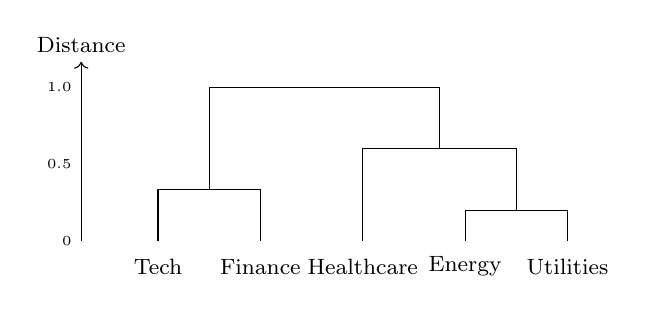
\begin{tikzpicture}[scale=0.65]
    % Simplified dendrogram
    \node at (0,-0.5) {\footnotesize Tech};
    \node at (2,-0.5) {\footnotesize Finance};
    \node at (4,-0.5) {\footnotesize Healthcare};
    \node at (6,-0.5) {\footnotesize Energy};
    \node at (8,-0.5) {\footnotesize Utilities};

    % First level merges
    \draw (0,0) -- (0,1) -- (2,1) -- (2,0);
    \draw (1,1) -- (1,1.5);

    \draw (4,0) -- (4,0.8);

    \draw (6,0) -- (6,0.6) -- (8,0.6) -- (8,0);
    \draw (7,0.6) -- (7,1.2);

    % Second level
    \draw (4,0.8) -- (4,1.8) -- (7,1.8) -- (7,1.2);
    \draw (5.5,1.8) -- (5.5,2.5);

    % Final merge
    \draw (1,1.5) -- (1,3) -- (5.5,3) -- (5.5,2.5);

    % Height labels
    \draw[->] (-1.5,0) -- (-1.5,3.5) node[above] {\footnotesize Distance};
    \node[left] at (-1.5,0) {\tiny 0};
    \node[left] at (-1.5,1.5) {\tiny 0.5};
    \node[left] at (-1.5,3) {\tiny 1.0};
  \end{tikzpicture}
  \end{center}

  \vspace{0.3em}
  \textbf{Typical findings:}
  \begin{itemize}
    \item Stocks often cluster by sector (industry effects)
    \item But not always! Data-driven clusters can cross sector boundaries
    \item Defensive stocks (utilities, staples) often group together
    \item Cyclical stocks (finance, industrials) form another group
  \end{itemize}
\end{frame}

%----------------------------------------------------------------------------------------

\begin{frame}{Portfolio Diversification via Clustering}

  \textbf{Traditional approach:} Equal-weight across sectors
  \begin{itemize}
    \item Problem: Sectors are arbitrary; stocks within sectors may be very different; ignores actual return correlations
  \end{itemize}

  \vspace{0.5em}
  \textbf{Clustering approach:} Diversify across \highlight{data-driven} groups
  \begin{itemize}
    \item Group stocks by how they actually move together
    \item Allocate across clusters, then within clusters
    \item Result: True diversification based on return behavior
  \end{itemize}

  \vspace{1em}
  \textbf{Why this matters:}
  \begin{itemize}
    \item Two ``tech'' stocks might behave very differently (Apple vs.\ Oracle)
    \item A ``consumer'' stock might move like tech (Amazon)
    \item Clustering reveals the \emph{true} groupings in your data
  \end{itemize}

  \vspace{0.5em}
  \begin{block}{Key Insight}
    Diversification means spreading risk across \highlight{uncorrelated} bets, not just different labels
  \end{block}
\end{frame}

%----------------------------------------------------------------------------------------

\begin{frame}{Example: Cluster-Based Allocation}

  \textbf{Suppose clustering reveals 3 groups among 9 stocks:}

  \vspace{0.5em}
  \begin{center}
  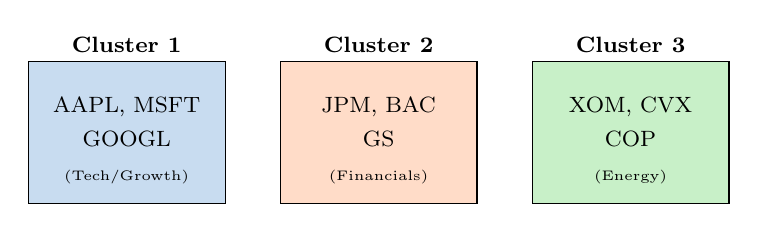
\begin{tikzpicture}[scale=0.8]
    % Cluster boxes
    \node[draw, fill=LightBlue, minimum width=2.5cm, minimum height=1.8cm] at (0,0) {};
    \node[draw, fill=LightOrange, minimum width=2.5cm, minimum height=1.8cm] at (4,0) {};
    \node[draw, fill=LightGreen, minimum width=2.5cm, minimum height=1.8cm] at (8,0) {};

    % Labels
    \node at (0,1.4) {\footnotesize \textbf{Cluster 1}};
    \node at (4,1.4) {\footnotesize \textbf{Cluster 2}};
    \node at (8,1.4) {\footnotesize \textbf{Cluster 3}};

    % Stocks
    \node at (0,0.4) {\footnotesize AAPL, MSFT};
    \node at (0,-0.1) {\footnotesize GOOGL};
    \node at (4,0.4) {\footnotesize JPM, BAC};
    \node at (4,-0.1) {\footnotesize GS};
    \node at (8,0.4) {\footnotesize XOM, CVX};
    \node at (8,-0.1) {\footnotesize COP};

    % Characteristics
    \node at (0,-0.7) {\tiny (Tech/Growth)};
    \node at (4,-0.7) {\tiny (Financials)};
    \node at (8,-0.7) {\tiny (Energy)};
  \end{tikzpicture}
  \end{center}

  \vspace{0.5em}
  \textbf{Simple cluster-based allocation:}
  \begin{enumerate}
    \item Allocate equally across clusters: 33.3\% each
    \item Within each cluster, equal-weight the stocks: 11.1\% per stock
  \end{enumerate}

  \vspace{0.5em}
  \textbf{Compare to naive equal-weight (11.1\% each):}
  \begin{itemize}
    \item If Tech cluster has 3 stocks but is highly correlated internally...
    \item ...you're putting 33\% in one ``bet'' without realizing it
    \item Cluster-aware allocation makes this explicit
  \end{itemize}
\end{frame}

%----------------------------------------------------------------------------------------
\section{Regime Detection with Clustering}
%----------------------------------------------------------------------------------------

\begin{frame}{Market Regimes}

  \textbf{Observation:} Market behavior changes over time

  \vspace{0.5em}
  \begin{itemize}
    \item \textbf{Bull markets:} Low volatility, positive drift, low correlations
    \item \textbf{Bear markets:} High volatility, negative drift, high correlations
    \item \textbf{Crisis periods:} Extreme volatility, correlations spike to 1
  \end{itemize}

  \vspace{1em}
  \textbf{Why does this matter?}
  \begin{itemize}
    \item Risk management: Volatility and correlations are regime-dependent
    \item Trading strategies: What works in one regime may fail in another
    \item Asset allocation: Defensive positioning in crisis, aggressive in recovery
  \end{itemize}

  \vspace{0.5em}
  \begin{block}{Idea}
    Use clustering to identify \highlight{time periods} with similar market conditions
  \end{block}
\end{frame}

%----------------------------------------------------------------------------------------

\begin{frame}{Clustering Time Periods}

  \textbf{Approach:} Cluster based on market characteristics

  \vspace{1em}
  \textbf{Features for each time period (e.g., month):}
  \begin{itemize}
    \item Market return
    \item Realized volatility
    \item Average correlation among stocks
    \item Spread between high and low beta stocks
    \item Credit spread, VIX, term spread
  \end{itemize}

  \vspace{1em}
  \textbf{Process:}
  \begin{enumerate}
    \item Compute features for each time period
    \item Standardize features
    \item Apply K-means or hierarchical clustering
    \item Label periods by cluster (``regimes'')
  \end{enumerate}
\end{frame}

%----------------------------------------------------------------------------------------

\begin{frame}{Example: Regime Detection Results}

  \textbf{Typical 3-regime structure:}

  \vspace{0.5em}
  \begin{center}
  \begin{tabular}{lccc}
    \toprule
    \textbf{Feature} & \textbf{Regime 1} & \textbf{Regime 2} & \textbf{Regime 3} \\
    & (Bull) & (Normal) & (Crisis) \\
    \midrule
    Market return & High (+) & Moderate & Low ($-$) \\
    Volatility & Low & Medium & High \\
    Avg correlation & 0.2--0.3 & 0.3--0.5 & 0.6--0.8 \\
    Frequency & 30\% & 55\% & 15\% \\
    \bottomrule
  \end{tabular}
  \end{center}

  \vspace{1em}
  \textbf{Applications:}
  \begin{itemize}
    \item \textbf{Conditional strategies:} Different model/allocation per regime
    \item \textbf{Risk budgeting:} Reduce risk when crisis regime detected
    \item \textbf{Factor timing:} Some factors work better in certain regimes
  \end{itemize}
\end{frame}

%----------------------------------------------------------------------------------------

\begin{frame}{Regime Detection Using Goyal-Welch Data}

  \textbf{Our data:} Same macroeconomic predictors from Weeks 2--3

  \vspace{0.5em}
  \textbf{Features we can use:}
  \begin{itemize}
    \item Market return (MktRf)
    \item Volatility proxy (svar --- stock variance)
    \item Term spread (tms)
    \item Default spread (dfy)
    \item Dividend yield (d\_y)
  \end{itemize}

  \vspace{0.5em}
  \textbf{Question:} Can we identify distinct market ``states'' in the data?

  \vspace{0.5em}
  \begin{block}{Exercise in Tutorial}
    Apply K-means clustering to monthly observations of GWZ variables. Do the clusters correspond to economically meaningful regimes?
  \end{block}
\end{frame}

%----------------------------------------------------------------------------------------
\section{PCA for Dimensionality Reduction in Prediction}
%----------------------------------------------------------------------------------------

\begin{frame}{The Curse of Dimensionality Revisited}

  \textbf{Recall from Week 2:} Many predictors create problems

  \vspace{0.5em}
  \begin{itemize}
    \item Overfitting: Model fits noise
    \item Multicollinearity: Correlated predictors, unstable estimates
    \item Computational cost: Large covariance matrices
  \end{itemize}

  \vspace{1em}
  \textbf{Solutions we've seen:}
  \begin{itemize}
    \item Regularization (Ridge, Lasso): Shrink or select coefficients
    \item Tree ensembles: Automatic feature selection
  \end{itemize}

  \vspace{0.5em}
  \textbf{Alternative approach:} \highlight{Reduce dimensions first}, then predict

  \vspace{0.3em}
  \begin{block}{PCA for Prediction}
    Replace $p$ original predictors with $k \ll p$ principal components
  \end{block}
\end{frame}

%----------------------------------------------------------------------------------------

\begin{frame}{Principal Component Regression (PCR)}

  \textbf{Procedure:}
  \begin{enumerate}
    \item Apply PCA to predictors $\mathbf{X}$, get $k$ principal components $\mathbf{F}$
    \item Regress target $\mathbf{y}$ on $\mathbf{F}$ instead of $\mathbf{X}$
    \[
    y_t = \gamma_0 + \gamma_1 F_{1t} + \gamma_2 F_{2t} + \cdots + \gamma_k F_{kt} + \varepsilon_t
    \]
  \end{enumerate}

  \vspace{1em}
  \textbf{Why does this help?}
  \begin{itemize}
    \item Fewer parameters: $k$ instead of $p$
    \item PCs are uncorrelated: No multicollinearity!
    \item Noise reduction: Drop PCs with small eigenvalues
  \end{itemize}

  \vspace{0.5em}
  \textbf{Important caveat:}
  \begin{itemize}
    \item PCA maximizes \emph{variance in $\mathbf{X}$}, not prediction of $\mathbf{y}$
    \item High-variance directions may not be the most predictive!
  \end{itemize}
\end{frame}

%----------------------------------------------------------------------------------------

\begin{frame}{PCR vs.\ Ridge: A Comparison}

  \textbf{Both shrink the effective number of parameters, but differently:}

  \vspace{1em}
  \begin{center}
  \begin{tabular}{lcc}
    \toprule
    & \textbf{PCR} & \textbf{Ridge} \\
    \midrule
    Approach & Drop less relevant PCs & Shrink all directions \\
    \addlinespace
    Shrinkage pattern & Discrete (keep or drop) & Continuous \\
    \addlinespace
    Uses $y$? & No (unsupervised) & Yes (supervised) \\
    \addlinespace
    Computation & Fast (closed form) & Fast (closed form) \\
    \addlinespace
    Interpretation & PCs may be interpretable & Original variables \\
    \bottomrule
  \end{tabular}
  \end{center}

  \vspace{0.5em}
  \textbf{Key insight:} Ridge shrinks \emph{more} in low-variance directions, which is often what we want. PCR drops them entirely.

  \vspace{0.3em}
  In practice, Ridge often outperforms PCR unless the factor structure in the data is very clear.
\end{frame}

%----------------------------------------------------------------------------------------

\begin{frame}{Application: Diffusion Index Forecasting}

  \textbf{Stock \& Watson (2002):} Use PCA for macroeconomic forecasting

  \vspace{0.5em}
  \textbf{Setting:}
  \begin{itemize}
    \item Many macro predictors (100+ series)
    \item Want to forecast inflation, output, etc.
    \item Too many predictors for standard regression
  \end{itemize}

  \vspace{0.5em}
  \textbf{Diffusion index approach:}
  \begin{enumerate}
    \item Apply PCA to macro predictors
    \item Keep first few PCs (``diffusion indices'')
    \item Use PCs as predictors in forecasting regression
  \end{enumerate}

  \vspace{0.5em}
  \textbf{Why ``diffusion''?}
  \begin{itemize}
    \item PCs summarize ``diffuse'' information across many series
    \item Each series contributes, none dominates
  \end{itemize}

  \vspace{0.3em}
  \textbf{Finance application:} Rapach, Strauss \& Zhou (2013) use diffusion indices for international return prediction
\end{frame}

%----------------------------------------------------------------------------------------
\section{Summary and Next Steps}
%----------------------------------------------------------------------------------------

\begin{frame}{Key Takeaways from Today}

  \begin{enumerate}
    \item \textbf{PCA for factor models:}
    \begin{itemize}
      \item Statistical factors from return covariances
      \item PC1 $\approx$ market, other PCs capture size/value/etc.
      \item Useful for covariance estimation, risk decomposition
    \end{itemize}

    \vspace{0.5em}
    \item \textbf{Clustering for portfolio construction:}
    \begin{itemize}
      \item Data-driven alternative to sector classification
      \item Correlation-based distance captures return co-movement
      \item Hierarchical clustering reveals structure
    \end{itemize}

    \vspace{0.5em}
    \item \textbf{Regime detection:}
    \begin{itemize}
      \item Cluster time periods by market characteristics
      \item Identifies bull/bear/crisis states
      \item Useful for conditional strategies
    \end{itemize}

    \vspace{0.5em}
    \item \textbf{PCR for prediction:}
    \begin{itemize}
      \item Reduce dimensions before regression
      \item Often inferior to Ridge (unsupervised vs.\ supervised)
    \end{itemize}
  \end{enumerate}
\end{frame}

%----------------------------------------------------------------------------------------

\begin{frame}{Readings and Next Steps}

\textbf{Readings for Today's Lecture:}
 \begin{itemize}
   \item James et al.\ (2023), Chapter 12 \hfill \textit{[Recomm.]}
   \item Hastie, Tibshirani \& Friedman (2009), Ch.\ 14.3, 14.5 \hfill \textit{[Supp.]}
    \item L\'{o}pez de Prado (2016), ``Building Diversified Portfolios that Outperform Out-of-Sample,'' \textit{JPM} \hfill \textit{[Supp.]}
    \item Stock \& Watson (2002), ``Forecasting Using Principal Components,'' \textit{JASA} \hfill \textit{[Supp.]}
    \item Rapach, Strauss \& Zhou (2013), ``International Stock Return Predictability,'' \textit{JF} \hfill \textit{[Supp.]}
  \end{itemize}

  \vspace{0.5em}
  \textbf{Coming up next Week:}
  \begin{itemize}
    \item Model interpretability and explainability
    \begin{itemize}
      \item Feature importance methods
     \item SHAP values
      \item Partial dependence plots
    \end{itemize}
    \item Why interpretability matters for finance and regulation
  \end{itemize}
\end{frame}

%----------------------------------------------------------------------------------------

\begin{frame}[plain]
  \centering
  \vfill
  {\Large Questions?}
  \vfill
\end{frame}

\end{document}
